   \begin{MyInnerSplitBox}{Year 8 and below}
      You have a chess board from which two diagonally opposite squares have been removed. You also have thirty-one dominoes, each of which can cover two squares of the chess board. Can the dominoes be arranged so that they cover all sixty-two squares of the chess board? If so, how? If not, why not?
      \iftoggle{SOLUTION}{%conditional output begin
      \begin{MySolutionBox}
        You can try proving that the thirty-one dominoes will cover the sixty-two squares but it is easier to find a solution if you start by trying to show the puzzle cannot be solved.\\
      Notice that two diagonally opposite squares are always the same colour, and that a domino must always cover two squares of \emph{different} colours.\\
      Therefore the problem cannot be solved because there are too few black squares.
      \end{MySolutionBox}
    }{}%conditional output end
      \tcblower
      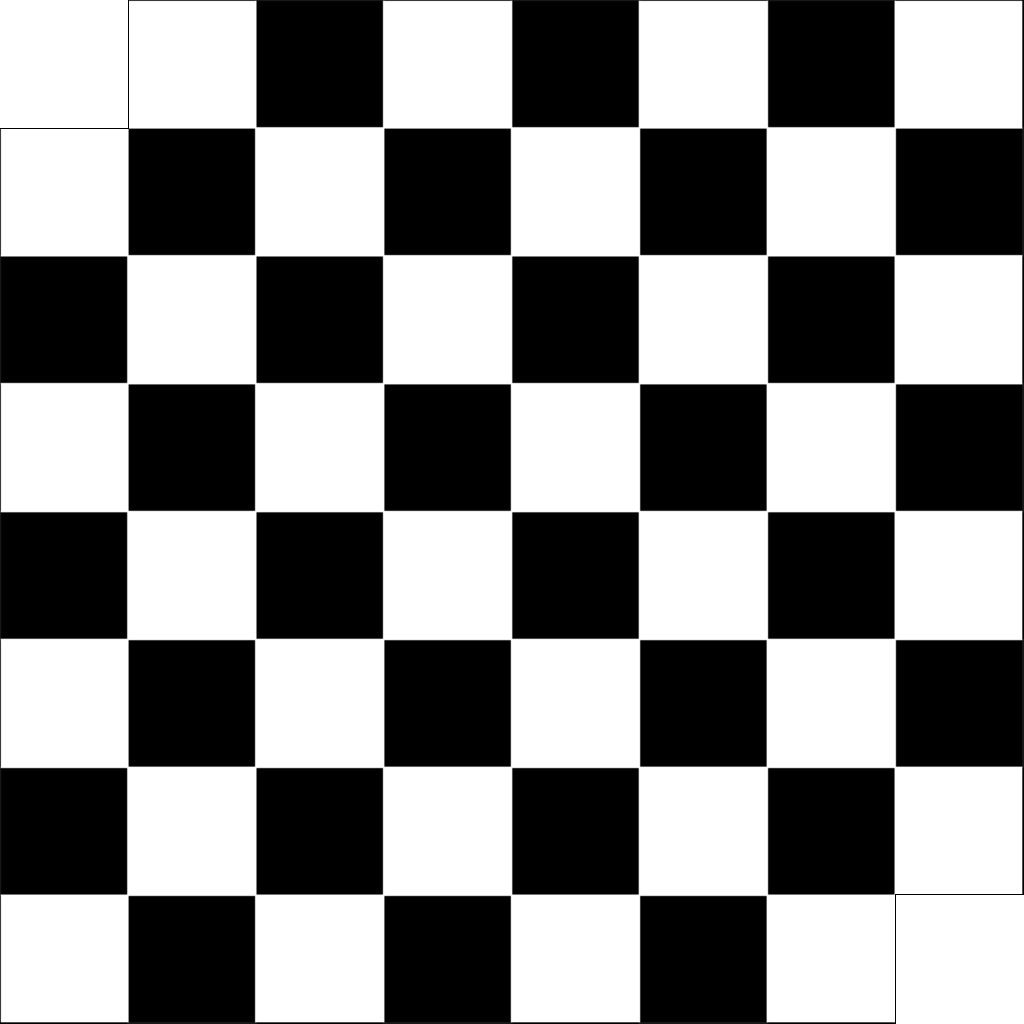
\includegraphics[width=\linewidth]{images/bwchess-2.jpg}%
    \end{MyInnerSplitBox}

